
\chapter{算法通用概念}

\section{CFL}

对于波动方程, 有关键参数 Courant number $C$:
\begin{equation}
    C = u \frac{\Delta t}{\Delta x}
\end{equation}

CFL (Courant–Friedrichs–Lewy) condition 的定义基于 Courant number:
\begin{equation}
    C = u \frac{\Delta t}{\Delta x} \leq C_{max}
\end{equation}




\section{convergence rate}

收敛率 (convergence rate) 是基于误差定义的。为了测试收敛率, 我们需要构造一系列的算例, 让每个算例的时间或者空间网格都比上一个算例的网格更精细。收敛率的测试依赖于假设:

\begin{equation}
    E = C_t \Delta t^r + C_x \Delta x^p
\end{equation}

其中 $E$ 是数值误差, $C_t$, $C_x$, $r$ 和 $p$ 是常数。$r$ 是时间上的收敛率, $p$ 是空间上的收敛率。比如当我们采用中心差分的离散方法, 我们期待 $r=p=2$ (根据截断误差的推导)。并且, 通常来说, $C_t$ 和 $C_x$ 的值的大小, 我们是不关心的。

% 还有一种误差的简化表示法。根据 Courant number $C= c\frac{\Delta t}{\Delta x}$, 并令 $h=\Delta t$, 我们有:

% $$
% E = C_t \Delta t^r + C_x \Delta x^r = C_t h^r + C_x \left(\frac{c}{C}\right)^r h^r = Dh^r \\
% D = C_t + C_x \left(\frac{c}{C}\right)^r
% $$

当我们计算误差的时候, 首先, 定义一个初始的空间步长 $h_0$, 然后定义随后的$h$:
\begin{equation}
    h_i = 2^{-i} h_0, \quad i=0,1,2,...,m
\end{equation}
一共有 $0,1,...,m$ : $m+1$ 这么多个算例。

对于每一个算例, 我们都记录 $E$ 和 $h$。 常见的 $E$ 有两种选择方法, $\ell^2$ norm 或者 $\ell^\infty$ norm:

\begin{equation}
\begin{aligned}
&E=\left\|e_{i}^{n}\right\|_{\ell^{2}}=\left(\Delta t \Delta x \sum_{n=0}^{N_{t}} \sum_{i=0}^{N_{x}}\left(e_{i}^{n}\right)^{2}\right)^{\frac{1}{2}}, \quad e_{i}^{n}=u_{\mathrm{e}}\left(x_{i}, t_{n}\right)-u_{i}^{n} \\
&E=\left\|e_{i}^{n}\right\|_{\ell^{\infty}}=\max _{i, n}\left|e_{n}^{i}\right|
\end{aligned}
\end{equation}


另外一种方式是记录单一时间步骤上的误差 $\ell^2$ 或 $\ell^\infty$, 比如在最后一个时间步上 ($n=N_t$):
\begin{equation}
\begin{aligned}
&E=\left\|e_{i}^{n}\right\|_{\ell^{2}}=\left(\Delta x \sum_{i=0}^{N_{x}}\left(e_{i}^{n}\right)^{2}\right)^{\frac{1}{2}}, \quad e_{i}^{n}=u_{\mathrm{e}}\left(x_{i}, t_{n}\right)-u_{i}^{n}, \\
&E=\left\|e_{i}^{n}\right\|_{\ell^{\infty}}=\max _{0 \leq i \leq N_{x}}\left|e_{i}^{n}\right| .
\end{aligned}
\end{equation}

有了误差的定义, 我们就可以计算收敛率了。令 $E_i$ 和 $h_i$ 对应于相应算例的误差和 step, 则: $E_i = Dh_i^r$, 针对两次连续的算例, 有:
\begin{equation}
    \begin{aligned}
        E_{i+1} &= Dh_{i+1}^r \\
        E_i &= Dh_i^r
    \end{aligned}
\end{equation}
两次算例的 $E_i$ 相除以消去 $D$, 有收敛率:
\begin{equation}
    r_i = \frac{\ln\left( \frac{E_{i+1}}{i}\right)}{\ln \left(\frac{h_{i+1}}{h_i}\right)}
\end{equation}

对于 $0,1,...,m$ 这样 $m+1$ 个算例, 一共有 $m$ 个$r_i, \quad i=0,1,...,m-1$。对于一些方程, 收敛率是可以解析的算出来的, 从而方便 benchmark. 比如对于的波动方程, 中心差分, 我们期待随着 $i$ 的增加 $r_i$ 收敛到 $2$.


\section{Accuracy}

当我们说一种离散格式具有 $p$ 阶精度 (accuracy) 的时候, 我们在说这种格式的误差有:
\begin{equation}
    E \propto h^p
\end{equation}
其中 $h$ 是网格步长。

所以对于一种数值格式, 当用 log-log plot 画出误差 vs 步长时, 我们可以发现直线的斜率就是精度 $p$:
\begin{equation}
    \begin{aligned}
        E(h) &\approx C h^p \\
        \mathrm{lg} |E(h)| &\approx \mathrm{lg} C + p\mathrm{lg} h
    \end{aligned}
\end{equation}

这就是为什么描述精度的时候喜欢用 log-log plot:
\begin{figure}[!hbtp]
    \centering
    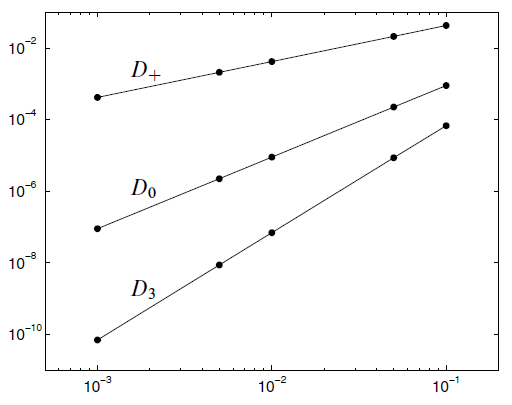
\includegraphics[width=0.7\textwidth]{figs/accuracy_temp.png} 
    \caption{描述精度示意图}
\end{figure}



